\subsection{Energiekalibration}
Für beide Detektoren wird ein Zusammenhang zwischen den Kanälen des MCA und der dem Signal entsprechenden Energie hergestellt. Dazu wird zunächst an die aufgenommenen \SI{511}{\kilo\electronvolt} Linien eine Gaußfunktion
\begin{align}
  N(n)=A \exp \left( -\frac{(n-\mu)}{2 \sigma^2} \right)
  \label{eq:gauss}
\end{align}
mit Gnuplot angepasst. Die resultierenden Parameter sind
\begin{align*}
  A_l&=195,4 \pm 0,9\\
  \mu_l&=7469,1 \pm 0,9\\
  \sigma_l&=261,1 \pm 0,8\\
  A_r&=168 \pm 1\\
  \mu_r&=6669 \pm 1\\
  \sigma_r&=227 \pm 1
\end{align*}
Die Spektren mit den angepassten Regressionskurven sind in Abbildung \ref{fig:511} zu sehen. \newpage
\begin{figure}[h]
  \centering
  \begin{subfigure}[h]{0.5\textwidth}
    \centering
    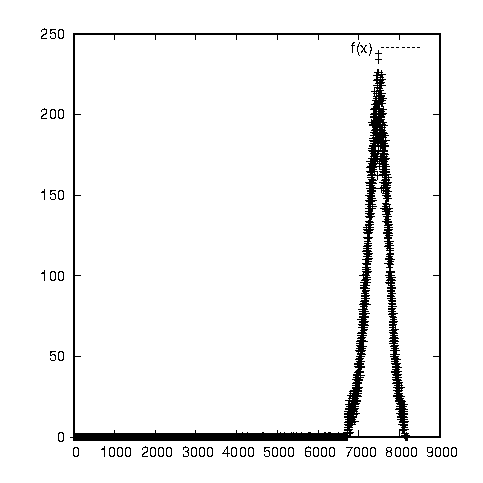
\includegraphics[width=0.9\textwidth]{data/Energiespektren/na_kal_links.eps}
    \subcaption{linker Detektor}
    \label{fig:511_links}
  \end{subfigure}%
  \begin{subfigure}[h]{0.5\textwidth}
    \centering
    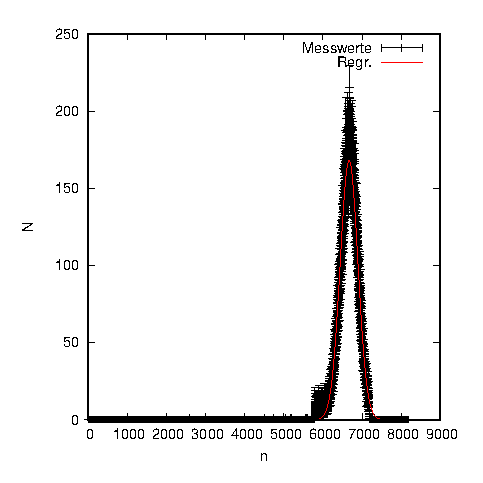
\includegraphics[width=0.9\textwidth]{data/Energiespektren/na_kal_rechts.eps}
    \subcaption{rechter Detektor}
    \label{fig:511_rechts}
  \end{subfigure}
  \caption{mit beiden Detektoren aufgenommene \SI{511}{\kilo\electronvolt} Linien}
  \label{fig:511}
\end{figure}

In den aufgenommenen Spektren von $^{133}$Ba sind sieben Peaks zu erkennen. An die Spektren wird eine Superposition von sieben Gaußkurven (siehe Gleichung \ref{eq:gauss}) und einer Gerade $a\cdot n+b$ angepasst. Die Spektren mit den angepassten Funktionen sind in Abbildung \ref{fig:ba_kal} zu sehen. Die Parameter der Regressionskurven befinden sich im Anhang in Tabelle \ref{tab:ba_links} und \ref{tab:ba_rechts}. 
\begin{figure}[h!]
  \centering
  \begin{subfigure}[h]{0.5\textwidth}
    \centering
    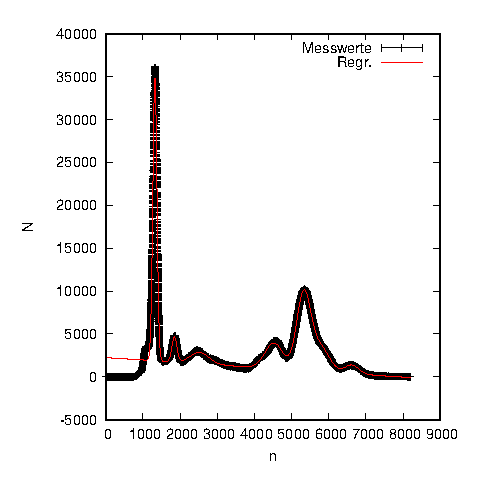
\includegraphics[width=0.9\textwidth]{data/Energiespektren/links_ba_cfd_kal.eps}
    \subcaption{linker Detektor}
    \label{fig:ba_kal_links}
  \end{subfigure}%
  \begin{subfigure}[h]{0.5\textwidth}
    \centering
    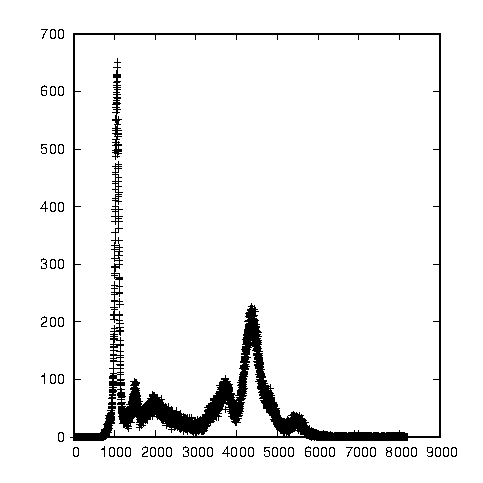
\includegraphics[width=0.9\textwidth]{data/Energiespektren/rechts_ba_cfd_kal.eps}
    \subcaption{rechter Detektor}
    \label{fig:ba_kal_rechts}
  \end{subfigure}
  \caption{mit beiden Detektoren aufgenommenes Spektrum von $^{133}$Ba}
  \label{fig:ba_kal}
\end{figure}

Nun werden die Peaks den bekannten Emissionslinien zugeordnet. Die Literaturwerte für die Zuordnung stammen aus \cite{baspektrum}. Zunächst ist anzumerken, dass ein Peak vor Peak 1, der dessen Höhe noch übetraf, von einem Röntgenübergang stammt. Dieser ist hier allerdings nicht relevant und wurde mit dem SCA ausselektiert. Folgende Energien können mit großer Sicherheit zugeordnet werden:
\begin{align*}
  E_1&=\SI{81}{\kilo\electronvolt}\\
  E_4&=\SI{303}{\kilo\electronvolt}\\
  E_5&=\SI{356}{\kilo\electronvolt}.
\end{align*}
Die restlichen Peaks können, trotz Hinzunahme der Amplituden und dem Vergleich mit den Übergangswahrscheinlichkeiten, nicht eindeutig dem Spektrum zugeordnet werden und werden deshalb nicht für die Energiekalibration berücksichtigt. Die \SI{511}{\kilo\electronvolt} Linie wird für die Kalibration mit einbezogen. Für beide Detektoren wird eine Funktion $E(n)=a\cdot n+b$ angepasst\footnote{Als Fehler für die jeweilige Kanalnummer wird $\sigma$ verwendet.}. Die resultierenden Parameter sind
\begin{align*}
  a_l&=\SI[separate-uncertainty=true]{0.0694 \pm 0.0004}{\kilo\electronvolt}\\
  b_l&=\SI[separate-uncertainty=true]{-11 \pm 1}{\kilo\electronvolt}\\
  a_r&=\SI[separate-uncertainty=true]{0,080 \pm 0,003}{\kilo\electronvolt}\\
  b_r&=\SI[separate-uncertainty=true]{-3 \pm 5}{\kilo\electronvolt}.
\end{align*}
Die angepassten Regresionsgeraden sind in Abbildung \ref{fig:energiekal} zu sehen.
\begin{figure}[h]
  \centering
  \begin{subfigure}[h]{0.5\textwidth}
    \centering
    \includegraphics[width=0.9\textwidth]{data/Energiespektren/energiekal_links.eps}
    \subcaption{linker Detektor}
    \label{fig:energiekal_links}
  \end{subfigure}%
  \begin{subfigure}[h]{0.5\textwidth}
    \centering
    \includegraphics[width=0.9\textwidth]{data/Energiespektren/energiekal_rechts.eps}
    \subcaption{rechter Detektor}
    \label{fig:energiekal_rechts}
  \end{subfigure}
  \caption{Regressionsgeraden für Energiekalibration}
  \label{fig:energiekal}
\end{figure}

\subsubsection{Energieauflösung}
Mit den Parametern der Energiekalibration und der einzelnen Peaks kann das Auflösungsvermögen bei der jeweiligen Energie über
\begin{align*}
  R=\frac{\Delta E}{E}=\frac{a\sigma 2\sqrt{2\ln(2)}}{a\mu+b}
\end{align*}
berechnet werden. $\Delta E$ ist dabei die Halbwertsbreite. Für beide Detektoren und die \SI{81}{\kilo\electronvolt}-, \SI{356}{\kilo\electronvolt}- und \SI{511}{\kilo\electronvolt}-Linie wird das Auflösungsvermögen bestimmt. Der jeweilige Fehler wird über die Gaußsche Fehlerfortpflanzung ermittelt. Das Ergebniss ist in Tabelle \ref{tab:aufloesungsvermoegen} zu sehen. \\
\begin{table}[h]
\centering
\caption{Auflösungsvermögen für jeweils drei Linien und beide Detektoren}
\label{tab:aufloesungsvermoegen}
\begin{tabular}{ccc}
\toprule
$E$ & $R_l/\%$ & $R_r/\%$\\
\midrule
\SI{81}{\kilo\electronvolt} & $11,1 \pm 0,1$ &$9,8 \pm 0,6$\\
\SI{356}{\kilo\electronvolt} & $8,6 \pm 0,1$ &$8,4 \pm 0,2$\\
\SI{511}{\kilo\electronvolt} & $8,42 \pm 0,04$ &$8,06 \pm 0,08$\\
\bottomrule
\end{tabular}
\end{table}

Es ist zu erkennen, dass das Auflösungsvermögen mit steigender Energie besser (also $R$ kleiner) wird. Außerdem hat der rechte Detektor eine bessere Auflösung.

\subsubsection{Energieschwellen}
Mit dem ermittelten Zusammenhang von Kanal und Energie kann zu jeder eingestellten Schwelle die entsprechende Energie ermittelt werden. Dazu wird für die vier Spektren aus Abbildung \ref{fig:511} und \ref{fig:ba_kal} abgelesen, bei welchem Kanal die Detektion von Ereignissen anfängt bzw. aufhört und anschließend die Kanalnummer zu der entsprechenden Energie umgerechnet (siehe Tabelle \ref{tab:intervalle}). Ein dauerhaft auftretender Untergrund, der vereinzelt für Detektionen von einem Ereignis (bei SCA) oder 1-10 Ereignissen (bei CFD) pro Kanal sorgt, wird nicht berücksichtigt. \\

\begin{table}[h]
\centering
\caption{Auflösungsvermögen für jeweils drei Linien und beide Detektoren}
\label{tab:intervalle}
\begin{tabular}{ccc}
\toprule
Spektrum & Kanalintervall & Energieintervall/\si{\kilo\electronvolt}\\
\midrule
$^{22}$Na, linker Detektor & [6727 ; 8132] &[$456 \pm 3$ ; $553 \pm 3$]\\ 
$^{22}$Na, rechter Detektor & [5782 ; 7182] & [$460 \pm 18$ ; $572 \pm 22$]\\
$^{133}$Ba, linker Detektor & [698 ; 8145] &[$37 \pm 1$ ; $554 \pm 3$]\\ 
$^{133}$Ba, rechter Detektor & [790 ; 5837] & [$60 \pm 6$ ; $464 \pm 18$]\\
\bottomrule
\end{tabular}
\end{table}

Die unteren Intervallgrenzen der Spektren von $^{133}$Ba bestätigen noch einmal, dass die Röntgenlinie bei etwa \SI{31}{\kilo\electronvolt} abgeschnitten wurde.
